\chapter{Integração Redmine e Activiti BPM}\label{chp:integracao_redmine_activiti}

\section{Introdução}\label{sec:integracao_intro}

A condução de processo simples no Redmine foi um sucesso. No entanto, encontramos dificuldades para automatizar processos mais complexos utilizando este sistema. Isto seria possível apenas com o desenvolvimento de plugins ou mudanças no código-fonte principal, ambas as opções custosas, arriscadas e imanuteníveis a longo prazo. Além disso, as funcionalidades que teríamos que desenvolver no Redmine para possibilitar a condução de processos mais complexos já existem nos BPMS, criados exatamente para este tipo de demanda. 

Utilizar apenas um BPMS contudo não se mostrou a melhor opção, pois perderíamos o excelente controle de permissões do Redmine, bem como a geração automática de formulários e a facilidade de criar um processo simples. 
Neste capítulo será apresentada a solução para os problemas citados acima: a integração entre o Redmine e o Activiti BPM, o BPMS escolhido para esta implementação.

\section{Motivos para integração}\label{sec:cenario-integracao}

A utilização do Redmine como gerenciador de processos torna-se limitada, como foi descrito no Capítulo \ref{chp:redmine}, já que ele não possui efetivamente um motor de processos BPM. Ainda assim, a possibilidade de extensão e desenvolvimento de novas funcionalidades no Redmine através de plugins sugere que o mesmo possa ser aperfeiçoado para o atendimento de processos mais complexos, ao mesmo tempo em que suas vantagens de portal e atendimento de processos mais simples são mantidos.

Com o objetivo de estender o Redmine para atender fluxos de trabalho mais complexos, torna-se necessário o desenvolvimento de um motor de processos mais robusto que possibilite novas opções e configurações de fluxos de trabalho na ferramenta. Entretanto, uma solução deste porte acaba por convergir em problemas solucionados por ferramentas BPMS, que permitem a modelagem e execução de processos complexos.

A utilização de BPMS para a automatização de processos de negócio traz diversas vantagens, conforme apresentado na seção \ref{sec:automatizacao-processos-bpms}. Entre elas, utilizar um sistema que implementa as funcionalidades previstas na notação BPMN, que permitem a condução de processos complexos, e por isto reduz a necessidade do desenvolvimento de funcionalidades específicas. 

Boa parte das aplicações BPMS mais robustas oferecem algum tipo de portal, onde ocorrem basicamente as interações com as tarefas humanas, e também APIs para manipulação dos processos, o que permite a integração com diferentes interfaces e aplicações. Entretanto, nem sempre esses portais possuem uma interface tão amigável para o usuário, ou são adaptados a dispositivos móveis como \textit{smartphones} ou \textit{tablets}, ou são de fácil customização. Essas são características positivas encontradas no Redmine, que conta com mais de 50 temas prontos para uso na lista oficial\cite{redmine_themes}, além de possuir uma estrutura bem organizada para customização e criação de novos \textit{layouts}. 

O Redmine também possui um excelente suporte à geração automática de formulários pela associação de campos customizados tipados às tarefas, como por exemplo datas, caixas de seleção e texto. Comparativamente, a implantação de processos mais simples pelo Redmine acaba sendo mais rápida e mais fácil de ser mantida do que em ferramentas BPMS, já que não é necessário nenhuma modelagem em notação específica, instalação de processos ou desenvolvimento de formulários; tudo é feito facilmente pela interface web. 

Neste sentido, torna-se interessante propor uma solução que aproveite todas as vantagens de portal e implantação de processos de negócio mais simples do Redmine, mas que também ofereça todo o poder e flexibilidade de modelagem de processos mais complexos oferecidos por ferramentas BPMS. Surge assim a proposta de uma solução integrada para a automatização de processos de negócio, através da junção do Redmine com uma ferramenta BPMS.

\section{Integração genérica}\label{sec:cenario-integracao-genérica}

 Pensando na possibilidade de utilizar qualquer plataforma BPMS integrada ao Redmine, decidimos avaliar a utilização de ferramentas ESB\cite{esb} de forma a facilitar a construção de uma interface única de comunicação com o Redmine. Conforme definido em publicação do O'Reilly\cite{oreilly_esb}, ESB é uma plataforma de integração baseada em padrões que combina mensagens, serviços web, transformação de dados e roteamento inteligente para conectar de forma confiável e coordenar a interação de um número significativo de aplicações e serviços. Assim, bastaria o trabalho de integrar o BPMS escolhido com este barramento, e assim o Redmine estaria capacitado a orquestrar fluxos de trabalho mais complexos utilizando qualquer BPMS de mercado. A Figura \ref{fig:arquitetura_integracao_generica_redmine_bpm}  apresenta o modelo de arquitetura proposto para a integração genérica do Redmine com BPMS.

\begin{figure}[H]
\centering
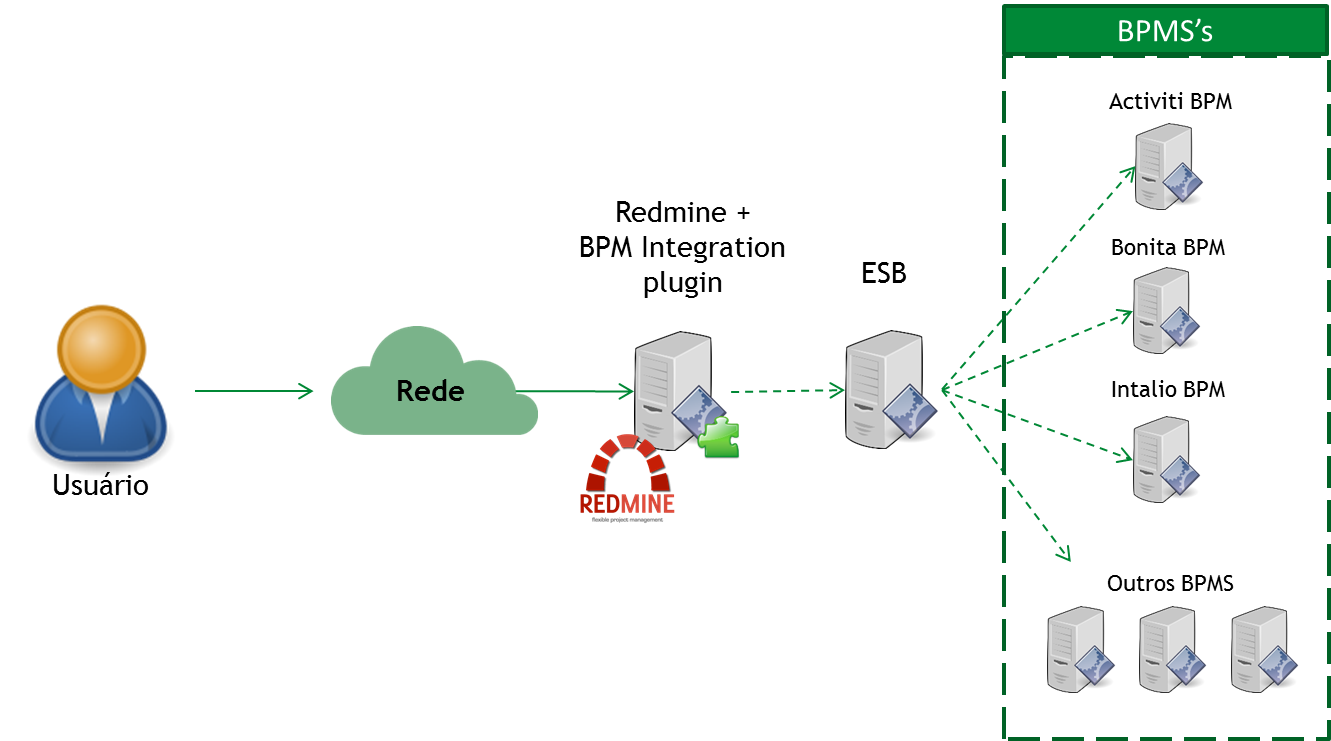
\includegraphics[width=1\textwidth]{imagens/arquitetura_proposta_inicialmente_bpm_integration.png}
\caption{Arquitetura proposta de integração genérica entre Redmine e BPMS's}
\label{fig:arquitetura_integracao_generica_redmine_bpm}
\end{figure}

Iniciamos o desenvolvimento deste barramento através da escolha de um ESB e pelo menos dois BPMS para validar a construção desta interface. Para o ESB, optamos pelo Mule ESB\cite{mule} que possui uma versão gratuita e está posicionado como uma das melhores ferramentas do seguimento de integração empresarial, segundo o quadrante mágico anual da Gartner\cite{mule_gartner}. Para o BPMS, optamos por duas ferramentas com versões gratuitas, desenvolvidas na linguaguem Java e com uma boa interface REST\cite{rest}: Activiti BPM\cite{bpm_activiti} e Bonita BPM\cite{bpm_bonita}.

Possuir uma boa API REST\cite{rest} é um ponto importante, pois é uma interface simples e muito usada, o que facilita utilizar a mesma estrutura para comunicação do ESB com os BPMS, além de ampliar o número de BPMS que poderíamos incluir posteriormente, pois muitos deles possuem uma interface REST.

O primeiro serviço escolhido para modelagem no barramento foi o responsável por disparar um novo processo no BPMS. Consistiria basicamente na disponibilização de um serviço REST, com parâmetros comuns às APIs de ambos os BPMS para que um novo processo fosse iniciado na plataforma escolhida. Apesar de um esforço considerável para a construção deste primeiro serviço, o mesmo foi desenvolvido com sucesso.  

Entretanto, este piloto foi suficiente para identificarmos logo no início que haveria um grande esforço para a construção deste barramento. Para implementar o serviço citado acima, foi necessário estudar a fundo os serviços implementados pela interface REST de cada BPMS e percebemos que haviam muitas diferenças entre eles. Devido a estas diferenças percebemos que não seria possível construir uma comunicação genérica entre o ESB e os BPMS, e exigiria uma alta complexidade. Percebemos fundamentalmente que esta solução exigiria um altíssimo esforço de desenvolvimento e modelagem, e que nos afastaríamos do objetivo central deste trabalho, que é prover um motor de processos mais complexo para o Redmine. Além disso, se tivéssemos que desenvolver uma estrutura nova de comunicação para cada BPMS, a camada de interface do ESB deixava de fazer sentido.

Em razão disso optamos por uma solução de menor complexidade, mas que provesse o ganho almejado com a integração do BPMS ao Redmine.

\section{Integração Redmine e Activiti BPM}\label{sec:activiti-bpm}

Dada a complexidade de criação de uma interface genérica de integração do Redmine com todos os BPMS, decidimos implementar a integração do Redmine com um BPMS específico de mercado. 

Para a escolha do BPMS de mercado, estabelecemos alguns critérios. O motor deveria ser gratuito e de código aberto, estando assim alinhado com a proposta open-source do Redmine. Além disso, seria fundamental que a ferramenta fosse leve, extensível e com uma API de fácil utilização e boa documentação, possibilitando assim um rápido entendimento da plataforma e abertura para qualquer modificação ou extensão necessária na ferramenta. Seria desejável também que a ferramenta estivesse em constante evolução e fosse suportada por uma comunidade ativa e que pudesse oferecer suporte para dúvidas encontradas durante o processo de integração.

Ao avaliarmos as possibilidades existentes, identificamos uma ferramenta que se encaixava bastante nos critérios adotados, o Activiti BPM. O Activiti BPM é uma ferramenta de código aberto, compartilhado no GitHub\cite{activiti_github}, possui extensa documentação\cite{activiti-userguide} e dispobiliza uma API REST, arquitetura oficialmente adotada pelo \textit{framework} Ruby on Rails desde sua versão 2.0, lançada em dezembro de 2007\cite{rails_rest_support}, facilitando a comunicação com o Redmine, que é escrito nesta linguagem, além das razões citadas na seção \ref{sec:cenario-integracao-genérica}.

\subsection{Activiti BPM}\label{sec:activiti}
Criado em 2010 por ex-integrantes do projeto jBPM\cite{bpm_jbpm}, o Activiti BPM\cite{bpm_activiti} é um projeto de código aberto sob a licença Apache\cite{apache_license}, que proporciona um motor BPM leve, estável e de fácil integração. O Activiti BPM é desenvolvido na linguagem de programação Java\cite{java-history} e é facilmente integrável com aplicações existentes por sua leveza e API\cite{api} amigável, além de utilizar a notação BPMN 2.0 para a modelagem dos processos.

Nesta seção, vamos apresentar os componentes do Activiti BPM, os requisitos de software para seu funcionamento e informações sobre o ambiente de execução e modelagem do processo.

\subsubsection{Componentes}\label{sec:automatizacao_processos-gestao_processos}

O Activiti BPM é constituído por diversos componentes que possibilitam o aproveitamento do ecossistema BPM. Com exceção do \textit{Activiti Engine}, que constitui o módulo principal da ferramenta, todos os demais módulos são opcionais e dependem do cenário de utilização do BPMS.

A Figura \ref{fig:activiti_componentes} apresenta os componentes do Activiti BPM: \textit{Activiti Modeler}, \textit{Activiti Designer}, \textit{Activiti Kickstart}, \textit{Activiti Engine}, \textit{Activiti Explorer} e \textit{Activiti REST}. Os componentes são classificados nas categorias \textit{Modeling} (Modelagem), \textit{Runtime} (Tempo de Execução) e \textit{Management} (Gerenciamento).

\begin{figure}[H]
\centering
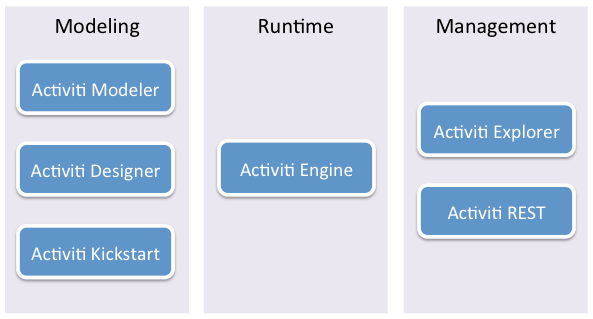
\includegraphics[width=1\textwidth]{imagens/activiti_components_overview.png}
\caption{Componentes do Activiti BPM\cite{activiti_componentes}}
\label{fig:activiti_componentes}
\end{figure}

\paragraph{Activiti Engine}\label{sec:automatizacao_processos-gestao_processos_activiti_engine}

O \textit{Activiti Engine} é o componente principal do Activiti BPM pois nele estão presentes o motor de funcionamento do BPM e as APIs para acesso e controle da ferramenta. Este componente é disponibilizado através de um simples arquivo JAR\cite{jar} (modelo de arquivo padrão para bibliotecas da linguagem Java). Sendo assim, o motor BPM pode ser facilmente utilizado em diferentes projetos Java através da inclusão dessa biblioteca como dependência.

\paragraph{Activiti Explorer}\label{sec:automatizacao_processos-gestao_processos_activiti_explorer}

O \textit{Activiti Explorer} é a interface web padrão com o usuário, disponibilizada para o controle e execução de processos. Através dessa interface, o usuário pode instalar novas definições de processos, iniciar ou cancelar processos, finalizar ou delegar tarefas. A Figura \ref{fig:activiti_explorer} mostra a janela do Activiti Explorer.

\begin{figure}[H]
\centering
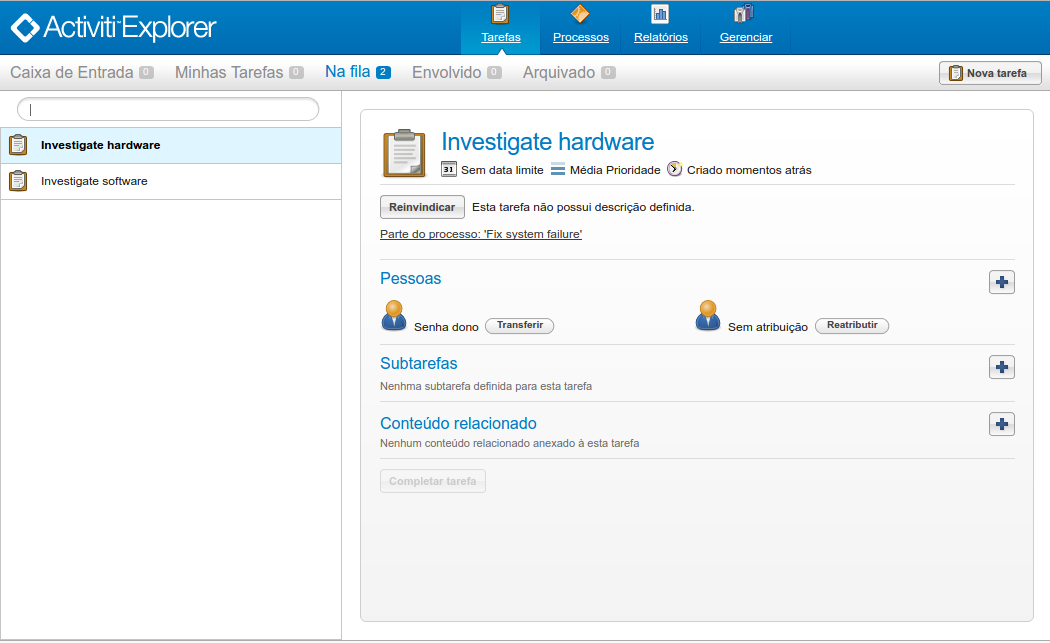
\includegraphics[width=1\textwidth]{imagens/activiti_explorer.png}
\caption{Activiti Explorer}
\label{fig:activiti_explorer}
\end{figure}

\paragraph{Activiti REST}\label{sec:automatizacao_processos-gestao_processos_activiti_rest}

O \textit{Activiti REST} disponibiliza o acesso às funcionalidades principais do Activiti através de uma interface REST. Isso simplifica o acesso às suas funcionalidades por diferentes linguagens de programação e facilita a integração com diferentes aplicações de interface com o usuário, como por exemplo aplicações para dispositivos móveis.

\paragraph{Activiti Designer}\label{sec:automatizacao_processos-gestao_processos_activiti_designer}

O \textit{Activiti Designer} é um plugin criado para a interface de desenvolvimento Eclipse. Ele permite ao analista ou desenvolvedor modelar processos na notação BPMN, e gera automaticamente a notação do processo em XML. A Figura \ref{fig:activiti_designer} mostra a IDE\cite{ide} \textit{Eclipse} já com o plugin \textit{Activiti Designer} instalado para a modelagem do processo.

\begin{figure}[H]
\centering
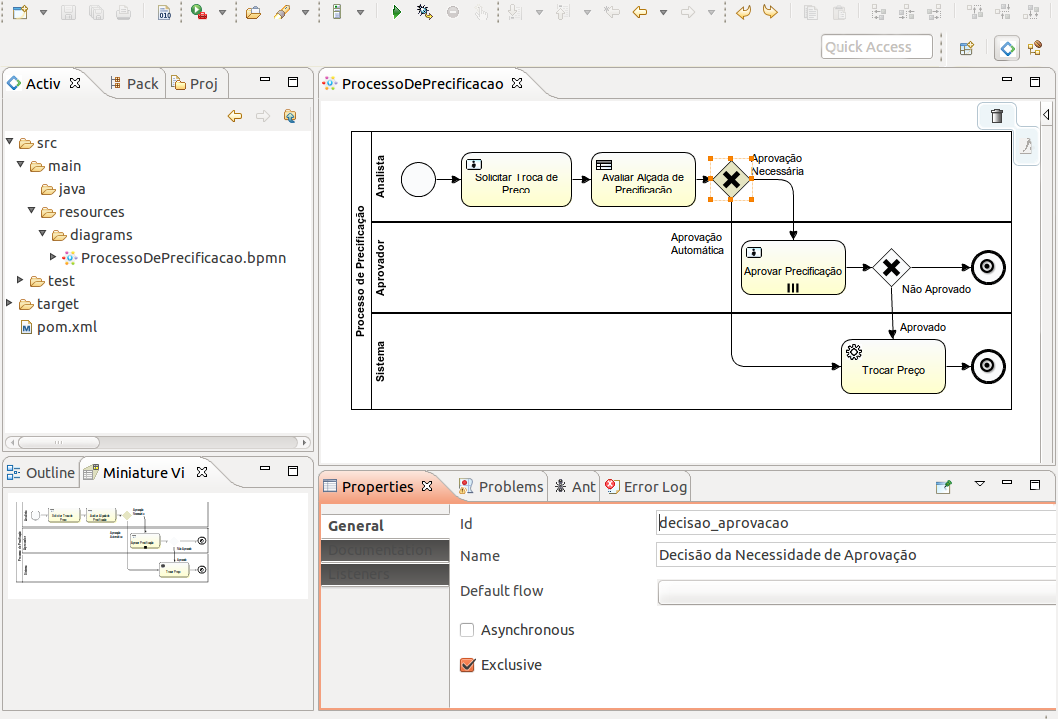
\includegraphics[width=1\textwidth]{imagens/activiti_designer.png}
\caption{Activiti Designer}
\label{fig:activiti_designer}
\end{figure}

\paragraph{Activiti Modeler}\label{sec:automatizacao_processos-gestao_processos_activiti_modeler}

O \textit{Activiti Modeler} possibilita a modelagem de processos BPMN 2.0 utilizando o browser. O Activiti Modeler não está mais em desenvolvimento ativo pela equipe principal, mas permanece disponível como parte da aplicação web Activiti Explorer.

\paragraph{Activiti Kickstart}\label{sec:automatizacao_processos-gestao_processos_activiti_kickstart}

O \textit{Activiti Kickstart} foi criado para facilitar a criação de processos \textit{adhoc} (sub-processos cujas tarefas podem ser executadas em qualquer ordem, várias vezes, ou mesmo puladas) através de uma interface web simples e intuitiva, sem que o usuário necessite conhecer BPMN, já que são utilizados tabelas e formulários simples para a definição do fluxo de trabalho. Seu objetivo é oferecer um meio rápido para construção de processos mais simples, reduzindo assim o custo e tempo investido na automatização desses processos.

\subsubsection{Requisitos de Software}\label{sec:automatizacao_processos-requisitos}

O Activiti BPM requer um ambiente Java JDK versão 6 ou superior para seu funcionamento. Além do ambiente Java configurado, também é necessário um banco de dados para suportar a persistência das informações dos processos. Uma variedade de bancos é suportada pelo BPMS, são eles: H2\cite{db_h2}, MySQL\cite{db_mysql}, Oracle\cite{db_oracle}, PostgreSQL\cite{db_postgres}, DB2\cite{db_db2} e SQL Server\cite{db_sqlserver}.

\subsubsection{Ambiente de Execução}\label{sec:automatizacao_processos-ambiente_desenvolvimento}

Existem basicamente duas possibilidades principais para configurar o ambiente de execução do Activiti BPM. A primeira opção é a inclusão da dependência do Activiti BPM em um projeto Java web, e a instalação do pacote WAR\cite{war} para execução em um servidor Java web. Outra opção, mais simples, é a utilização do pacote WAR já pronto para funcionamento, disponibilizado diretamente no site da ferramenta\cite{activiti_download}.

O arquivo disponibilizado no portal da ferramenta já inclui o \textit{Activiti Engine} e o \textit{Activiti Explorer} num único pacote pré-configurados com um banco de dados em memória H2\cite{h2_inmemory} que dá suporte ao seu funcionamento e não requer nenhuma configuração adicional, já que é um banco de dados \textit{in-memory}\cite{h2_inmemory}. Para iniciar a execução do BPMS, é necessária a instalação do artefato em um servidor Java como o Apache Tomcat 7\cite{tomcat7}.

Após a instalação do artefato e inicialização do Tomcat, o portal pode ser acessado através do endereço \textit{http://127.0.0.1:8080/activiti-explorer}, dado que o Tomcat tenha sido instalado na sua configuração padrão. A Figura \ref{fig:activiti_login} demonstra a tela de autenticação do \textit{Activiti Explorer}.

\begin{figure}[H]
\centering
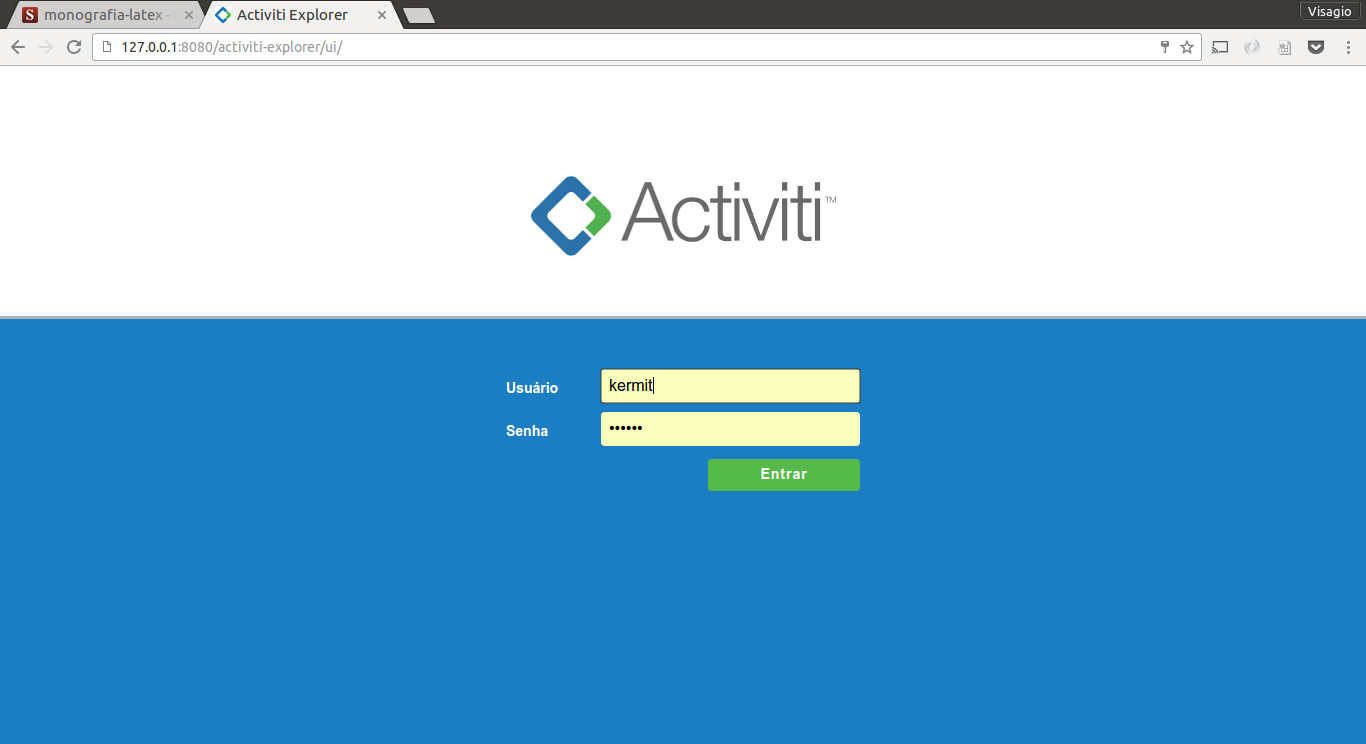
\includegraphics[width=0.9\textwidth]{imagens/activiti_login.png}
\caption{Login do Activiti Explorer}
\label{fig:activiti_login}
\end{figure}

\subsubsection{Modelagem do processo}\label{sec:automatizacao_processos-modelagem_processo}

Para a modelagem do processo, é necessária a instalação do plugin \textit{Activiti Designer} na ferramenta de desenvolvimento \textit{Eclipse}\cite{eclipse}. Mais detalhes sobre como proceder com a instalação do plugin estão disponíveis no guia de instalação disponível no site\cite{activiti_designer} do Activiti BPM.

Ao criar um novo diagrama através da opção de criar um novo \textit{Activiti Diagram}, o \textit{Activiti Designer} cria um arquivo \textit{.bpmn} e disponibiliza duas visões para a modelagem do processo. Uma aba visual, contendo o desenho do processo, e outra aba textual, com a notação em XML. Ambas as abas estão interligadas e podem ser utilizadas para a modelagem, sendo a visual mais simples para o desenvolvimento do processo.

Para a modelagem do processo na paleta visual, é necessário arrastar os componentes visuais dispostos na aba lateral a fim de obter a modelagem desejada do processo na notação BPMN.

Ao final da modelagem, o arquivo \textit{.bpmn} é gerado para ser utilizado na instalação do processo no motor de processos. A Figura \ref{fig:processo_precificacao} representa a modelagem 
do processo ilustrado na introdução deste trabalho utilizando o \textit{Activiti Designer} e já descrito na notação BPMN 2.0. O código gerado em XML pode ser consultado no apêndice \ref{code:process_bpmn}.

\begin{figure}[H]
\centering
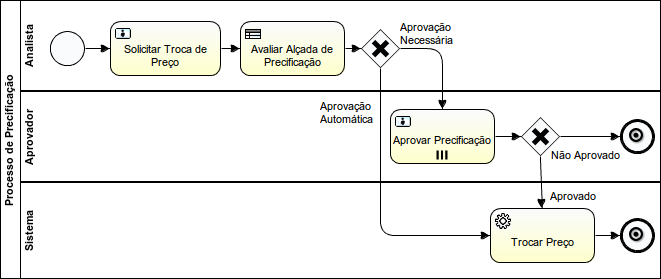
\includegraphics[width=1.0\textwidth]{imagens/ProcessoDePrecificacao}
\caption{Processo modelado no Activiti BPM}
\label{fig:processo_precificacao}
\end{figure}

\section{Customização do Redmine}\label{sec:integracao_redmine_activiti-implementacao}

Para atingir nosso objetivo de integração do Redmine com o Activiti BPM, criamos um plugin para o Redmine que possibilita a comunicação com o Activiti BPM. Chamamos este plugin de BPM Integration. Nas próximas sessões, descreveremos o processo de construção deste plugin e como utilizá-lo. Neste trabalho utilizamos a versão 3.1 do Redmine\cite{redmine31}.

\subsection{Arquitetura da solução}\label{sec:integracao_redmine_activiti_implementacao-arquitetura}

A integração proposta tem por objetivo centralizar o máximo de funcionalidades no Redmine, deixando transparente tanto para o usuário comum como o gestor a existência de um motor BPM por trás dele.

\begin{figure}[H]
\centering
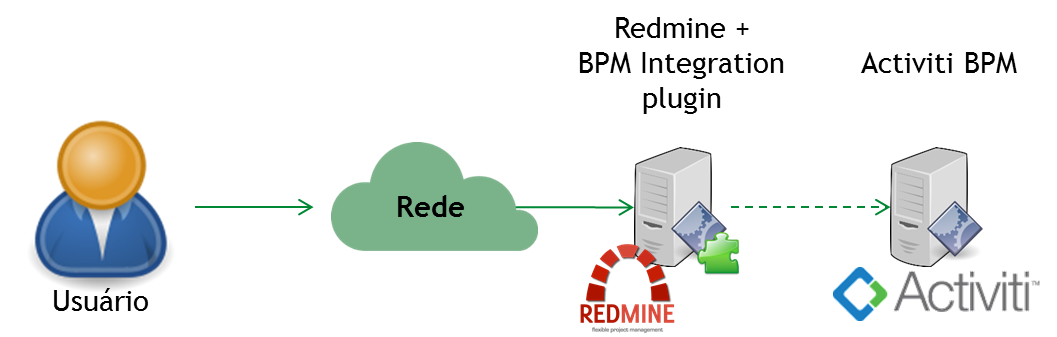
\includegraphics[width=1\textwidth]{imagens/arquitetura_desenvolvida_bpm_integration.png}
\caption{Arquitetura da integração entre Redmine e Activiti}
\label{fig:arquitetura_integracao_redmine_bpm}
\end{figure}

A Figura \ref{fig:arquitetura_integracao_redmine_bpm} ilustra a arquitetura da solução de integração proposta. O usuário continua a interagir diretamente com o Redmine da mesma maneira que fazia antes da criação do \textit{plugin}. O Redmine, então, se comunica com o Actitivi pela sua API disponibilizada através de um Web Service REST.

A abordagem utilizada visou concentrar todo o esforço de integração do lado do Redmine, sem a necessidade de customização do Activiti BPM, tornando transparente para ele, também, que o Redmine está sendo usado como sua interface com os usuários finais.
    
\subsection{Linguagens}\label{sec:integracao_redmine_activiti_implementacao_detalhes_desenvolvimento_linguagens}

O plugin desenvolvido para o Redmine foi implementado em Ruby\cite{ruby-lang}, utilizando a framework Rails\cite{rails}.
As modificações realizadas no Activiti BPM foram implementadas em Java, a linguagem em que este foi desenvolvido.

\subsection{Banco de dados}\label{sec:integracao_redmine_activiti_implementacao__bd}

O banco de dados utilizado neste trabalho foi o MySQL 5.7 por ser o banco de dados mais utilizado e testado com o Redmine pela comunidade.

\subsection{Comunicação entre o Redmine e Activiti}\label{sec:integracao_redmine_activiti_implementacao_sincronizacao}

Para possibilitar a integração entre o Activiti BPM e o Redmine, foi necessário construir no Redmine uma estrutura de dados que represente o modelo de dados do BPMS. Também foi preciso garantir a atualização das informações relativas ao andamento dos fluxos dos processos de forma que eles possam ser desempenhados corretamente através do Redmine. Assim, fez-se necessário o desenvolvimento de um mecanismo de sincronização entre as duas aplicações.

Toda a comunicação entre as duas ferramentas foi desenhada de forma que o Redmine funcionasse como uma interface do Activiti BPM. Portanto, o Redmine consome a API REST do BPMS para disparar ações ou ler informações do mesmo.

No restante desta seção apresentamos os detalhes da integração proposta: o tópico \ref{sec:integracao_redmine_activiti_sincronizacao-deploy_processo} descreve a utilização do Redmine para  a criação de novas definições de processos no Activiti BPM e como os novos dados são mapeados de volta para o Redmine; os tópicos \ref{sec:integracao_redmine_activiti_sincronizacao-inicializacao_processo} e \ref{sec:integracao_redmine_activiti_sincronizacao-finalizacao_human_task} mostram, respectivamente, como o Redmine é utilizado para iniciar novas instâncias de processos (relativos às definições previamente configuradas) e finalizar as tarefas em andamento. Por fim; os tópicos \ref{sec:integracao_redmine_activiti_sincronizacao-criacao_human_task} e \ref{sec:integracao_redmine_activiti_sincronizacao-status_processo} explicam como é feita a sincronização dos dados presentes no Activiti BPM para o Redmine, criando as novas tarefas e atualizando o \textit{status} dos processos até serem concluídos no BPMS.

\subsubsection{Definição de processo}\label{sec:integracao_redmine_activiti_sincronizacao-deploy_processo}

Para o Redmine assumir a função de interface principal do Activiti BPM foi desenvolvida uma funcionalidade do Activiti Explorer que permite ao usuário fazer a instalação de um processo através dele, uma ação que envia o arquivo da modelagem BPMN e disponibiliza o processo para ser iniciado. Esta funcionalidade dispara um serviço que acessa a API REST do Activiti BPM, executando uma requisição POST que efetivamente realiza a instalação, adicionando a modelagem do processo em questão à lista de definições de processos ativos que podem ser iniciados. 
Após executada a requisição POST, é iniciada uma rotina que busca a definição do processo recém criado. As informações do processo que são recuperadas consistem das tarefas humanas definidas, campos de formulário, variáveis de processo e outros detalhes.
A Figura \ref{fig:sync_deploy_process} ilustra a sequência de ações descritas acima.

\begin{figure}[H]
\centering
\includegraphics[width=0.6\textwidth]{imagens/sync_deploy_process.png}
\caption{Diagrama de sequência de instalação (deploy) de processo}
\label{fig:sync_deploy_process}
\end{figure}

Na Figura \ref{fig:process_list} é possível observar a lista de definições de processo apresentada no Redmine. Cada linha desta tabela representa um processo diferente que pode ser iniciado no Activiti BPM, resultando na criação de uma tarefa no Redmine associada ao respectivo tipo de tarefa configurado para o processo.

\begin{figure}[H]
\centering
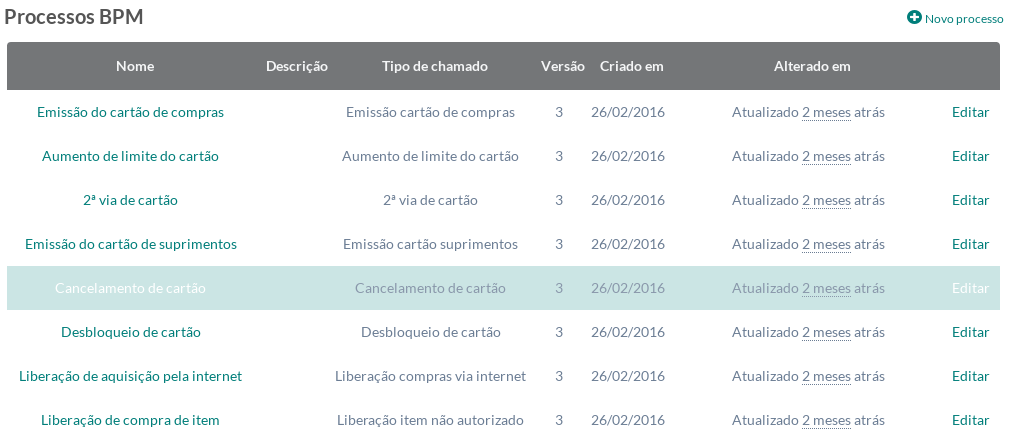
\includegraphics[width=1\textwidth]{imagens/plugin_process_list.png}
\caption{Lista de definições de processo disponíveis no Activiti BPM exibida na tela do plugin do Redmine}
\label{fig:process_list}
\end{figure}

\subsubsection{Inicialização de um processo}\label{sec:integracao_redmine_activiti_sincronizacao-inicializacao_processo}

Sempre que uma tarefa vinculada a um processo BPM é criada (configuração provida pelo plugin), é disparado um procedimento de sincronização ilustrado na Figura \ref{fig:start_process_diagram}. Esta vinculação é feita através da uma configuração na tela que pode ser acessada ao clicar em cada definição de processo da lista na tela exibida na Figura \ref{fig:process_list}. Este procedimento executa uma requisição à API REST do Activiti BPM que inicia uma nova instância de um processo no mesmo. A requisição carrega as informações da tarefa recém-criada, inclusive os valores dos campos customizados que foram mapeados para algum campo de formulário da definição de processo do BPMS. O status da tarefa do Redmine é, então, atualizado a partir do retorno do serviço do Activiti e é disparado o procedimento de sincronização de tarefas descrito na seção \ref{sec:integracao_redmine_activiti_sincronizacao-criacao_human_task}.

\begin{figure}[H]
\centering
\includegraphics[width=0.65\textwidth]{imagens/sync_start_process.png}
\caption{Diagrama de sequências ilustrando criação de processo no ActivitiBPM a partir do Redmine}
\label{fig:start_process_diagram}
\end{figure}


A Figura \ref{fig:new_issue} mostra a tela de criação de tarefas no Redmine responsável por disparar um novo processo no Activiti BPM do tipo "Emissão cartão suprimentos" usado como exemplo.

\begin{figure}[H]
\centering
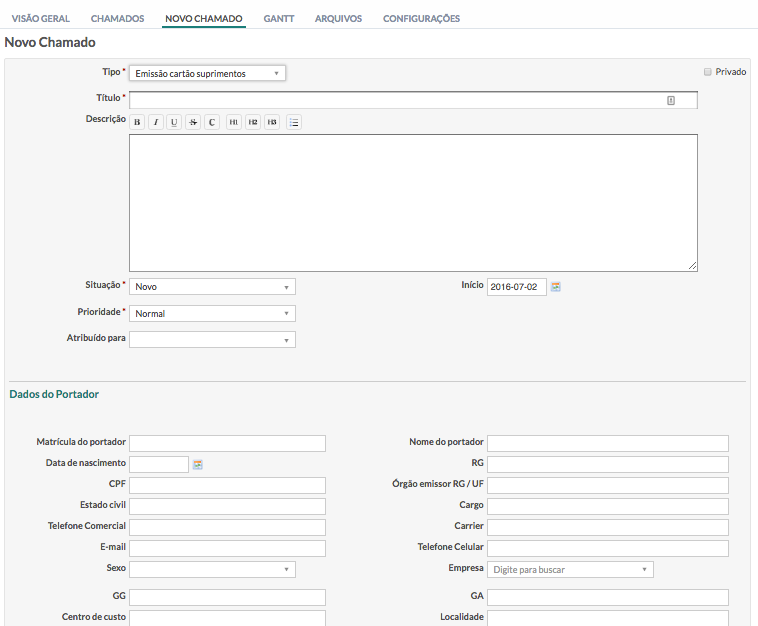
\includegraphics[width=1\textwidth]{imagens/redmine_new_issue.png}
\caption{Tela de criação de tarefas no Redmine}
\label{fig:new_issue}
\end{figure}

Os valores preenchidos para os campos padrão do Redmine são gravados no processo iniciado no Activiti BPM, bem como os campos personalizados que são configurados. Foi desenvolvida uma funcionalidade que permite ao usuário mapear cada campo personalizado para um campo presente no modelo do processo. A Figura \ref{fig:plugin_process_settings_variables} mostra a tela onde esta configuração é feita. Nesta mesma tela são configurados \underline{variáveis do processo},  \underline{estados de conclusão do processo} e \underline{mensagens de conclusão} e \underline{estados iniciais das tarefas do processo} no Redmine. 

Os campos citados acima são declaradas no XML de modelagem do processo na notação BPMN. O plugin BPM Integration lê estas variáveis através da API REST do Activiti BPM e monta esta tela de configuração.
As variáveis de processo são dados constantes utilizados ao longo do processo que são inicializadas com o valor preenchido nesta tela. O tipo de valor a ser preenchido para cada váriável depende de sua declaração, podendo ser uma situação (\ref{subsection:redmine-estrutura_basica-status}), um usuário, um grupo ou um campo personalizado (\ref{subsection:redmine-estrutura_basica-custom_fields}) cadastrado no Redmine ou um texto livre. Na configuração dos estados de conclusão o usuário deve preencher a situação correspondende a cada evento (\ref{sec:bpm-bpmn_objetos_fluxo}) de conclusão previsto no processo. Sempre que um processo é finalizado no Activiti BPM, o Redmine identifica e transiciona a situação para a situação configurada nesta tela. Também é possível configurar uma mensagem de conclusão padrão, que será preenchida como nota na tarefa do Redmine junto à mudança de situação. Em "Status inicial das tarefas do processo" o usuário configura a situação inicial para cada sub-tarefa que é criada durante o processo. Na seção \ref{sec:integracao_redmine_activiti_sincronizacao-criacao_human_task} explicaremos como as sub-tarefas são usadas para representar etapas do processo.

\begin{figure}[H]
\centering
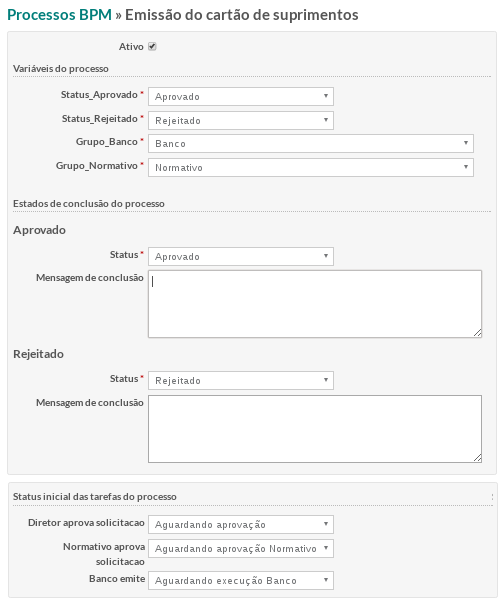
\includegraphics[width=0.65\textwidth]{imagens/plugin_process_settings1.png}
\caption{Tela de configurações do processo - Variáveis}
\label{fig:plugin_process_settings_variables}
\end{figure}

\begin{figure}[H]
\centering
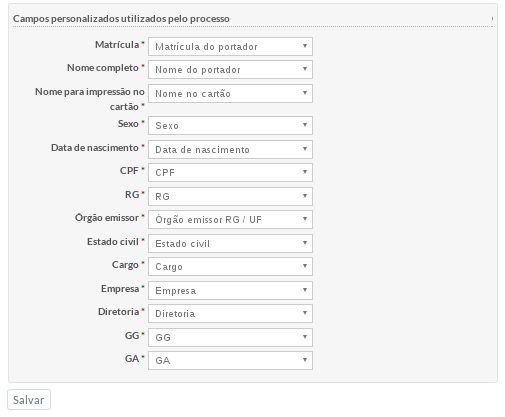
\includegraphics[width=0.65\textwidth]{imagens/plugin_process_settings2.png}
\caption{Tela de configurações do processo - Campos personalizados}
\label{fig:plugin_process_settings_form_fields}
\end{figure}

\subsubsection{Tarefas humanas}\label{sec:integracao_redmine_activiti_sincronizacao-criacao_human_task}

Chamaremos as tarefas que são realizadas por humanos, citadas na seção \ref{sec:bpm-bpmn_objetos_fluxo}, \underline{tarefas humanas}. Quando uma atividade deste tipo está presente na modelagem de um processo, significa que a etapa em questão deve ser realizada por uma pessoa. A interação do responsável pela tarefa com o processo é um dos pontos fortes do Redmine. Utilizando o plugin BPM Integration, as tarefas humanas do Activiti BPM são representadas no Redmine por sub-tarefas das tarefas que representam processos. Uma sub-tarefa nada mais é que uma hierarquia de tarefas, como mencionado na seção \ref{subsection:redmine-estrutura_basica-tarefa}.
Quando uma tarefa humana é criada no decorrer do processo, o Redmine precisa refletir isto, de modo que esta tarefa possa ser executada pelo ator correto e o processo siga seu curso. O espelhamento desta tarefa no Redmine é totalmente automatizado através de uma rotina do plugin BPM Integration que é executada periodicamente e verifica se existem tarefas humanas no Activiti BPM que não foram espelhadas no Redmine, e cria uma nova sub-tarefa. Os valores dos \underline{campos do processo} de uma tarefa são populados nos campos padrão e campos personalizados conforme configurados na tela exibida na Figura \ref{fig:plugin_process_settings_form_fields}. Esta rotina também é executada quando um novo processo é iniciado ou uma tarefa finalizada.

\begin{figure}[H]
\centering
\includegraphics[width=0.6\textwidth]{imagens/sync_create_tasks.png}
\caption{Diagrama de sequência de criação de tarefas do Activiti no Redmine}
\label{fig:sync_bpm_tasks}
\end{figure}

A Figura \ref{fig:sync_bpm_tasks} descreve este procedimento: primeiramente, o Redmine realiza uma consulta à API REST do Activiti para buscar as tarefas que estão em andamento, então verifica quais ainda não foram mapeadas para si, e, por fim, cria as novas tarefas, guardando referência da tarefa original do Activiti para que não sejam criadas novamente em uma futura reexecução do processo.

\subsubsection{Finalização de tarefas}\label{sec:integracao_redmine_activiti_sincronizacao-finalizacao_human_task}

Quando uma tarefa do Redmine é finalizada, é necessário concluir a sua contra-parte no Activiti, quando houver, dando seguimento ao fluxo do processo no motor BPM. A Figura \ref{fig:close_bpm_tasks} mostra a sequência de processamento realizada com a conclusão da tarefa no Redmine.

\begin{figure}[H]
\centering
\includegraphics[width=0.6\textwidth]{imagens/sync_close_tasks.png}
\caption{Diagrama de sequência de finalização de tarefas do Activiti pelo Redmine}
\label{fig:close_bpm_tasks}
\end{figure}

Após o usuário concluir a tarefa (transicionar para uma situação que representa a sua conclusão), o Redmine utiliza a API REST do Activiti para finalizar a tarefa correspondente no BPMS. Uma vez a tarefa concluída, os campos da tarefa principal do Redmine que representa o processo do Activiti são atualizados com as alterações realizadas na tarefa e são executados, em sequência, os \textit{jobs} de sincronização de tarefas e de processos, descritos nas seções \ref{sec:integracao_redmine_activiti_sincronizacao-criacao_human_task} e \ref{sec:integracao_redmine_activiti_sincronizacao-status_processo}, respectivamente.

\subsubsection{Atualização de processos}\label{sec:integracao_redmine_activiti_sincronizacao-status_processo}

O último tópico que necessita ser sincronizado é o \textit{}{status} do processo no Redmine para refletir o andamento do fluxo do processo no BPMS. Este procedimento é executado periodicamente para manter as tarefas do Redmine sempre atualizadas em relação ao Activiti.

\begin{figure}[H]
\centering
\includegraphics[width=0.6\textwidth]{imagens/sync_process_status.png}
\caption{Diagrama de sequência de sincronização de status do processo}
\label{fig:sync_process_status}
\end{figure}

A Figura \ref{fig:sync_process_status} mostra a sequência de execução desta sincronização. O Redmine consulta a API REST do Activiti para buscar os dados do andamento do processo. A partir dos dados obtidos é possível determinar se houve alteração na situação do processo ou ele foi terminado. Neste último caso, além de atualizar a situação do chamado no Redmine, também é escrita a mensagem de conclusão configurada no \textit{plugin}.

\section{Customização do Activiti BPM}\label{sec:integracao_redmine_activiti-implementacao-activiti}

A integração entre o Redmine e o Activiti BPM foi desenvolvida sob o aspecto de direcionar a maior parte das customizações para o lado do Redmine, uma vez que esta é apenas uma das possibilidades de interface com o motor de processos. Num cenário mais amplo de processos mais complexos, outros tipos de dispositivos ou sistemas poderiam realizar uma comunicação direta com os processos.

A API REST padrão oferecida pelo Activiti BPM foi utilizada para a integração entre as ferramentas, uma vez que é bem completa e oferece a maioria dos serviços necessários para a comunicação. Também contou a facilidade de chamadas a APIs REST pelo Ruby on Rails. 

Entretanto, identificamos a ausência de um serviço fundamental para integração entre as ferramentas. Esse serviço deveria retornar uma lista contendo as definições de tarefas contidas em um determinado processo, incluindo os campos disponíveis nos formulários das tarefas. Essa definição nos permitiria estabelecer a interface para o mapeamento dos campos do processo com os campos das tarefas do Redmine.

Sendo assim, foi necessário estendermos a API REST do Activiti BPM através da criação de uma classe Java representando um novo serviço, semelhante aos serviços existentes no seu código-fonte. Esse serviço consistiu no consumo de uma API Java já disponibilizada pelo Activiti BPM, mas ausente na API REST. O código-fonte pode ser consultado no apêndice \ref{code:task_definition_service}.